\section{Results \& Discussion }
\label{sec:results}

In this section, I shall cover the various results that I inferred while running the DAC V1.1 and DAC V2.0 system and discuss about my findings. In the first subsection we shall see how the DAC V1.1 system performed on running long times and the observations made while running it. In the second subsection we shall see how the DAC V2.0 system performed and the observations. 

\subsection{Observations from DAC V1.1 system}
\label{sec:dacv1.1obs}

\begin{figure}[H]
    \centering
    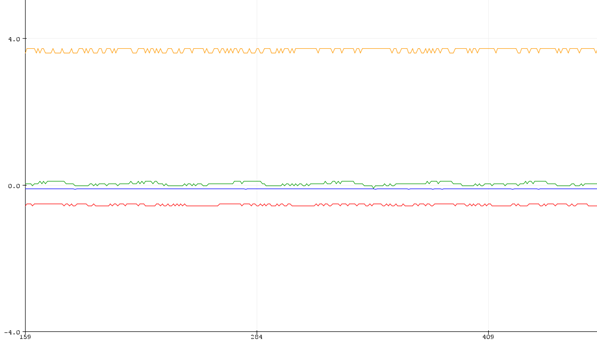
\includegraphics[scale = 1.2]{images/mywork/Sprint2/pressuresensor.png}
    \caption{Pressure sensor outputs : Blue - P1, Red - P2, Green - P3 and Yellow - P4}
    \label{fig:psensor}
\end{figure}


The DAC V1.1 system desorber can be seen in Figure \ref{fig:desorber}. Since the desorber components were already present. I conducted leak tests and running the system for sometime to see if there is any issue with the PEI pump or the vacuum compressor. A point to note is that the system was designed to produce 50 bar pressure but on running it is found that the $3^{rd}$ stage of the compressor isn't pumping at the designed pressure ratio. This can be seen in the Figure \ref{fig:psensor} where the maxmium pressure output from the 4 stage compressor system is only below 4 bar pressure. It can also be seen that the P1,P2 and P3 are all around 0 bar pressure line which is not at all a desired output.
\bigbreak 
It was concluded to be due to leaks being present in the compressor system. So, leak tests were conducted as seen in Figure \ref{fig:leaktest} to see if there were any bubbles moving due to leaked gases at the Swagelok joints of the compressor system but the compressor had passed the leak test. On further examination by Pim (the LIS student who built the system), he pointed out that one of the Swagelok joints were in inch standards and not in the metric standards that we were using throughout the the system. 

\begin{figure}[H]
    \centering
    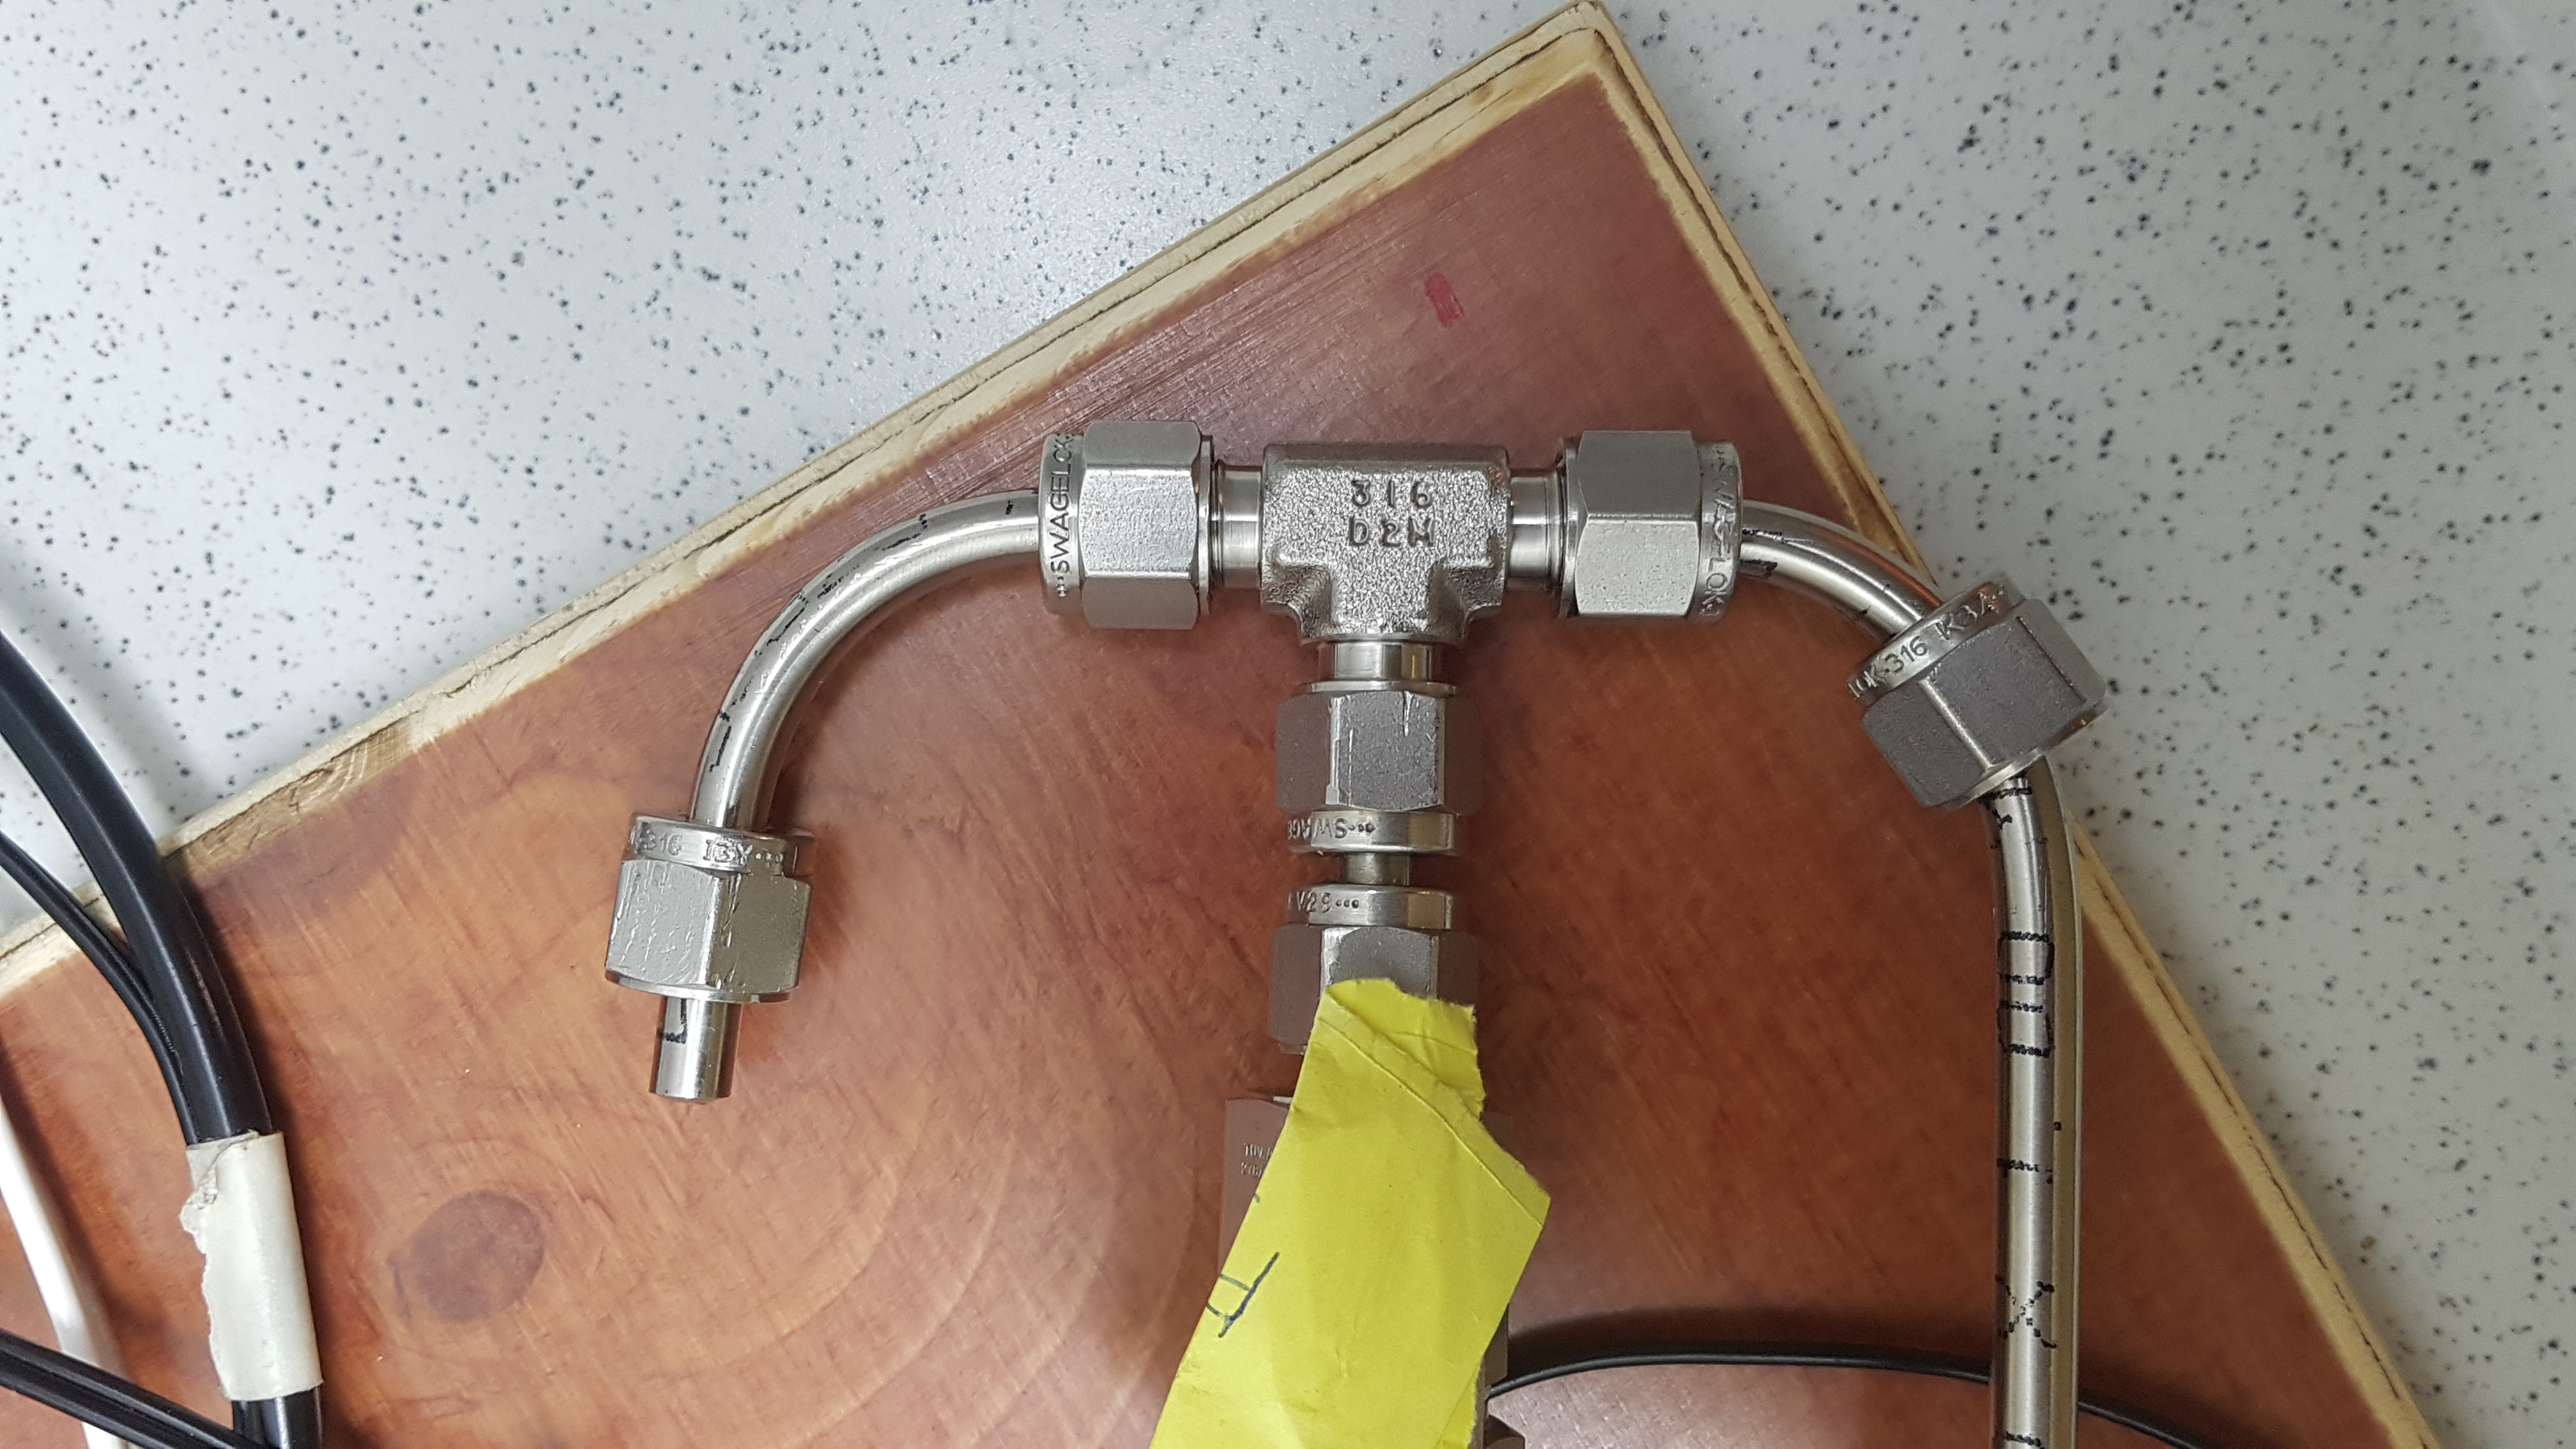
\includegraphics[width = \linewidth]{images/mywork/Sprint2/swagelok.jpg}
    \caption{Fixed the Swagelok joint}
    \label{fig:swagiss}
\end{figure}

In Figure \ref{fig:swagiss} the metric swagelok nuts are indicated by the small ring like feature below the octagonal feature used to hold the spanner. As seen in the figure, all the joints are fixed and made with metric bolts as per Pim's suggestion. Finally, the DAC system is complete and system is made to run. 

\subsubsection{Water testing}
\label{sec:watertest}

First, in order to ensure that there is no leaks in the system. Water was passed through the system - which was quite a bad idea since some of the water went into the vacuum compressor system. However, it turned out to be fine as all the water was cleared out. Once the water was all cleared out, PEI was passed into the system and made to run in the system and the system is closed. A proper flow of PEI was occurring with minimal to no leaks or spills. However, all the wiring was in a haphazard manner and I was told to make the electronic circuits into modules. Which was done using transparent boxes from Gamma store. Holes were created in the boxes so that wires can go from inside the box to outside the box and vice versa.
\bigbreak 
In Figure \ref{fig:dacsystem1.1}, we can see the complete DAC System V1.1 with all the components working together as one unit. In the background you can see the old broken down DAC System V1.0 of ZEF IV team. The following are the labelled components of the DAC system: 

\begin{itemize}
    \item 1 - DAC Absorber V1.1 
    \item 2 - DAC Desorber V1.1 
\end{itemize}

\begin{figure}[H]
    \centering
    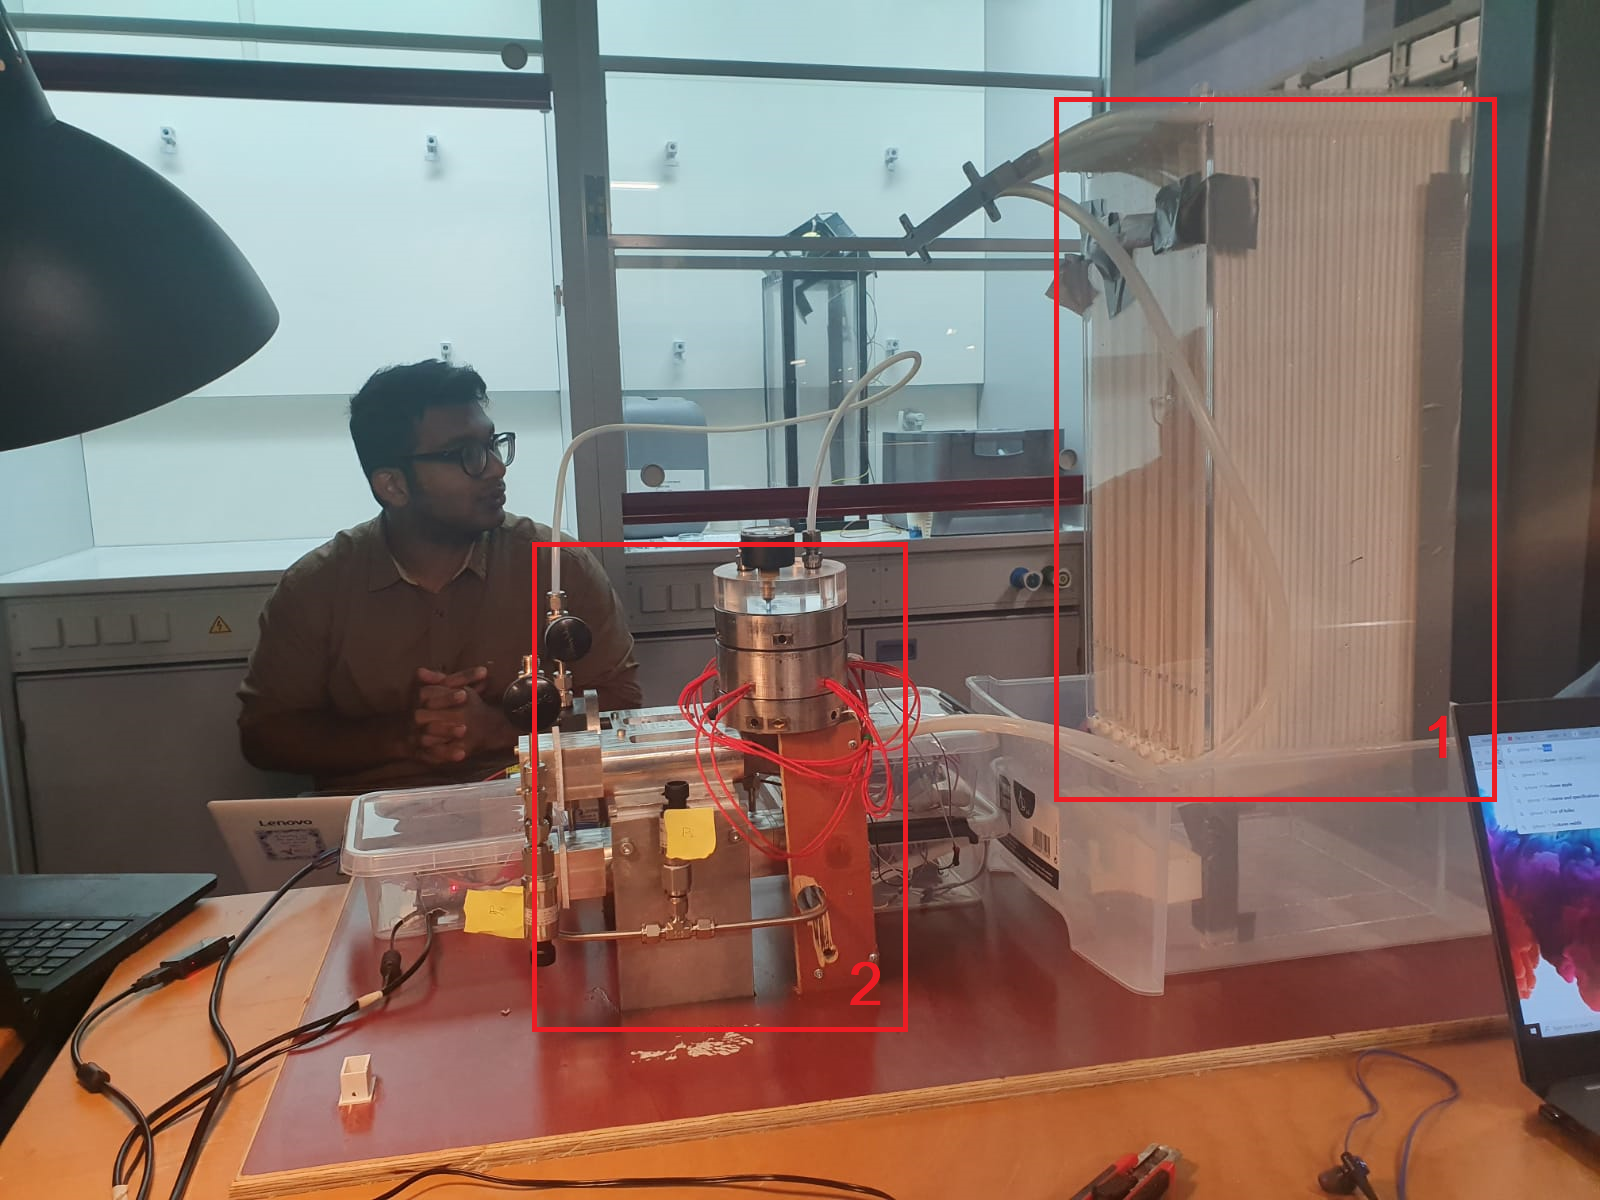
\includegraphics[scale = 0.45]{images/mywork/Sprint2/dacsystem1.png}
    \caption{The complete DAC System V1.1 }
    \label{fig:dacsystem1.1}
\end{figure}


\subsubsection{Running the DAC System V1.1 for long times with PEI}
\label{sec:obs}

We ran the DAC System V1.1 for about 7.23 hours cumulatively at varying RPMs of the PEI pump motor for various test conditions before the system broke. At first, we loaded PEI into the system from the desorbtion chamber without heating the desorbtion chamber. It can be seen in the Figure \ref{fig:peiloading}. This was done just to observe how PEI is flowing through the system. 

\begin{figure}[H]
    \centering
    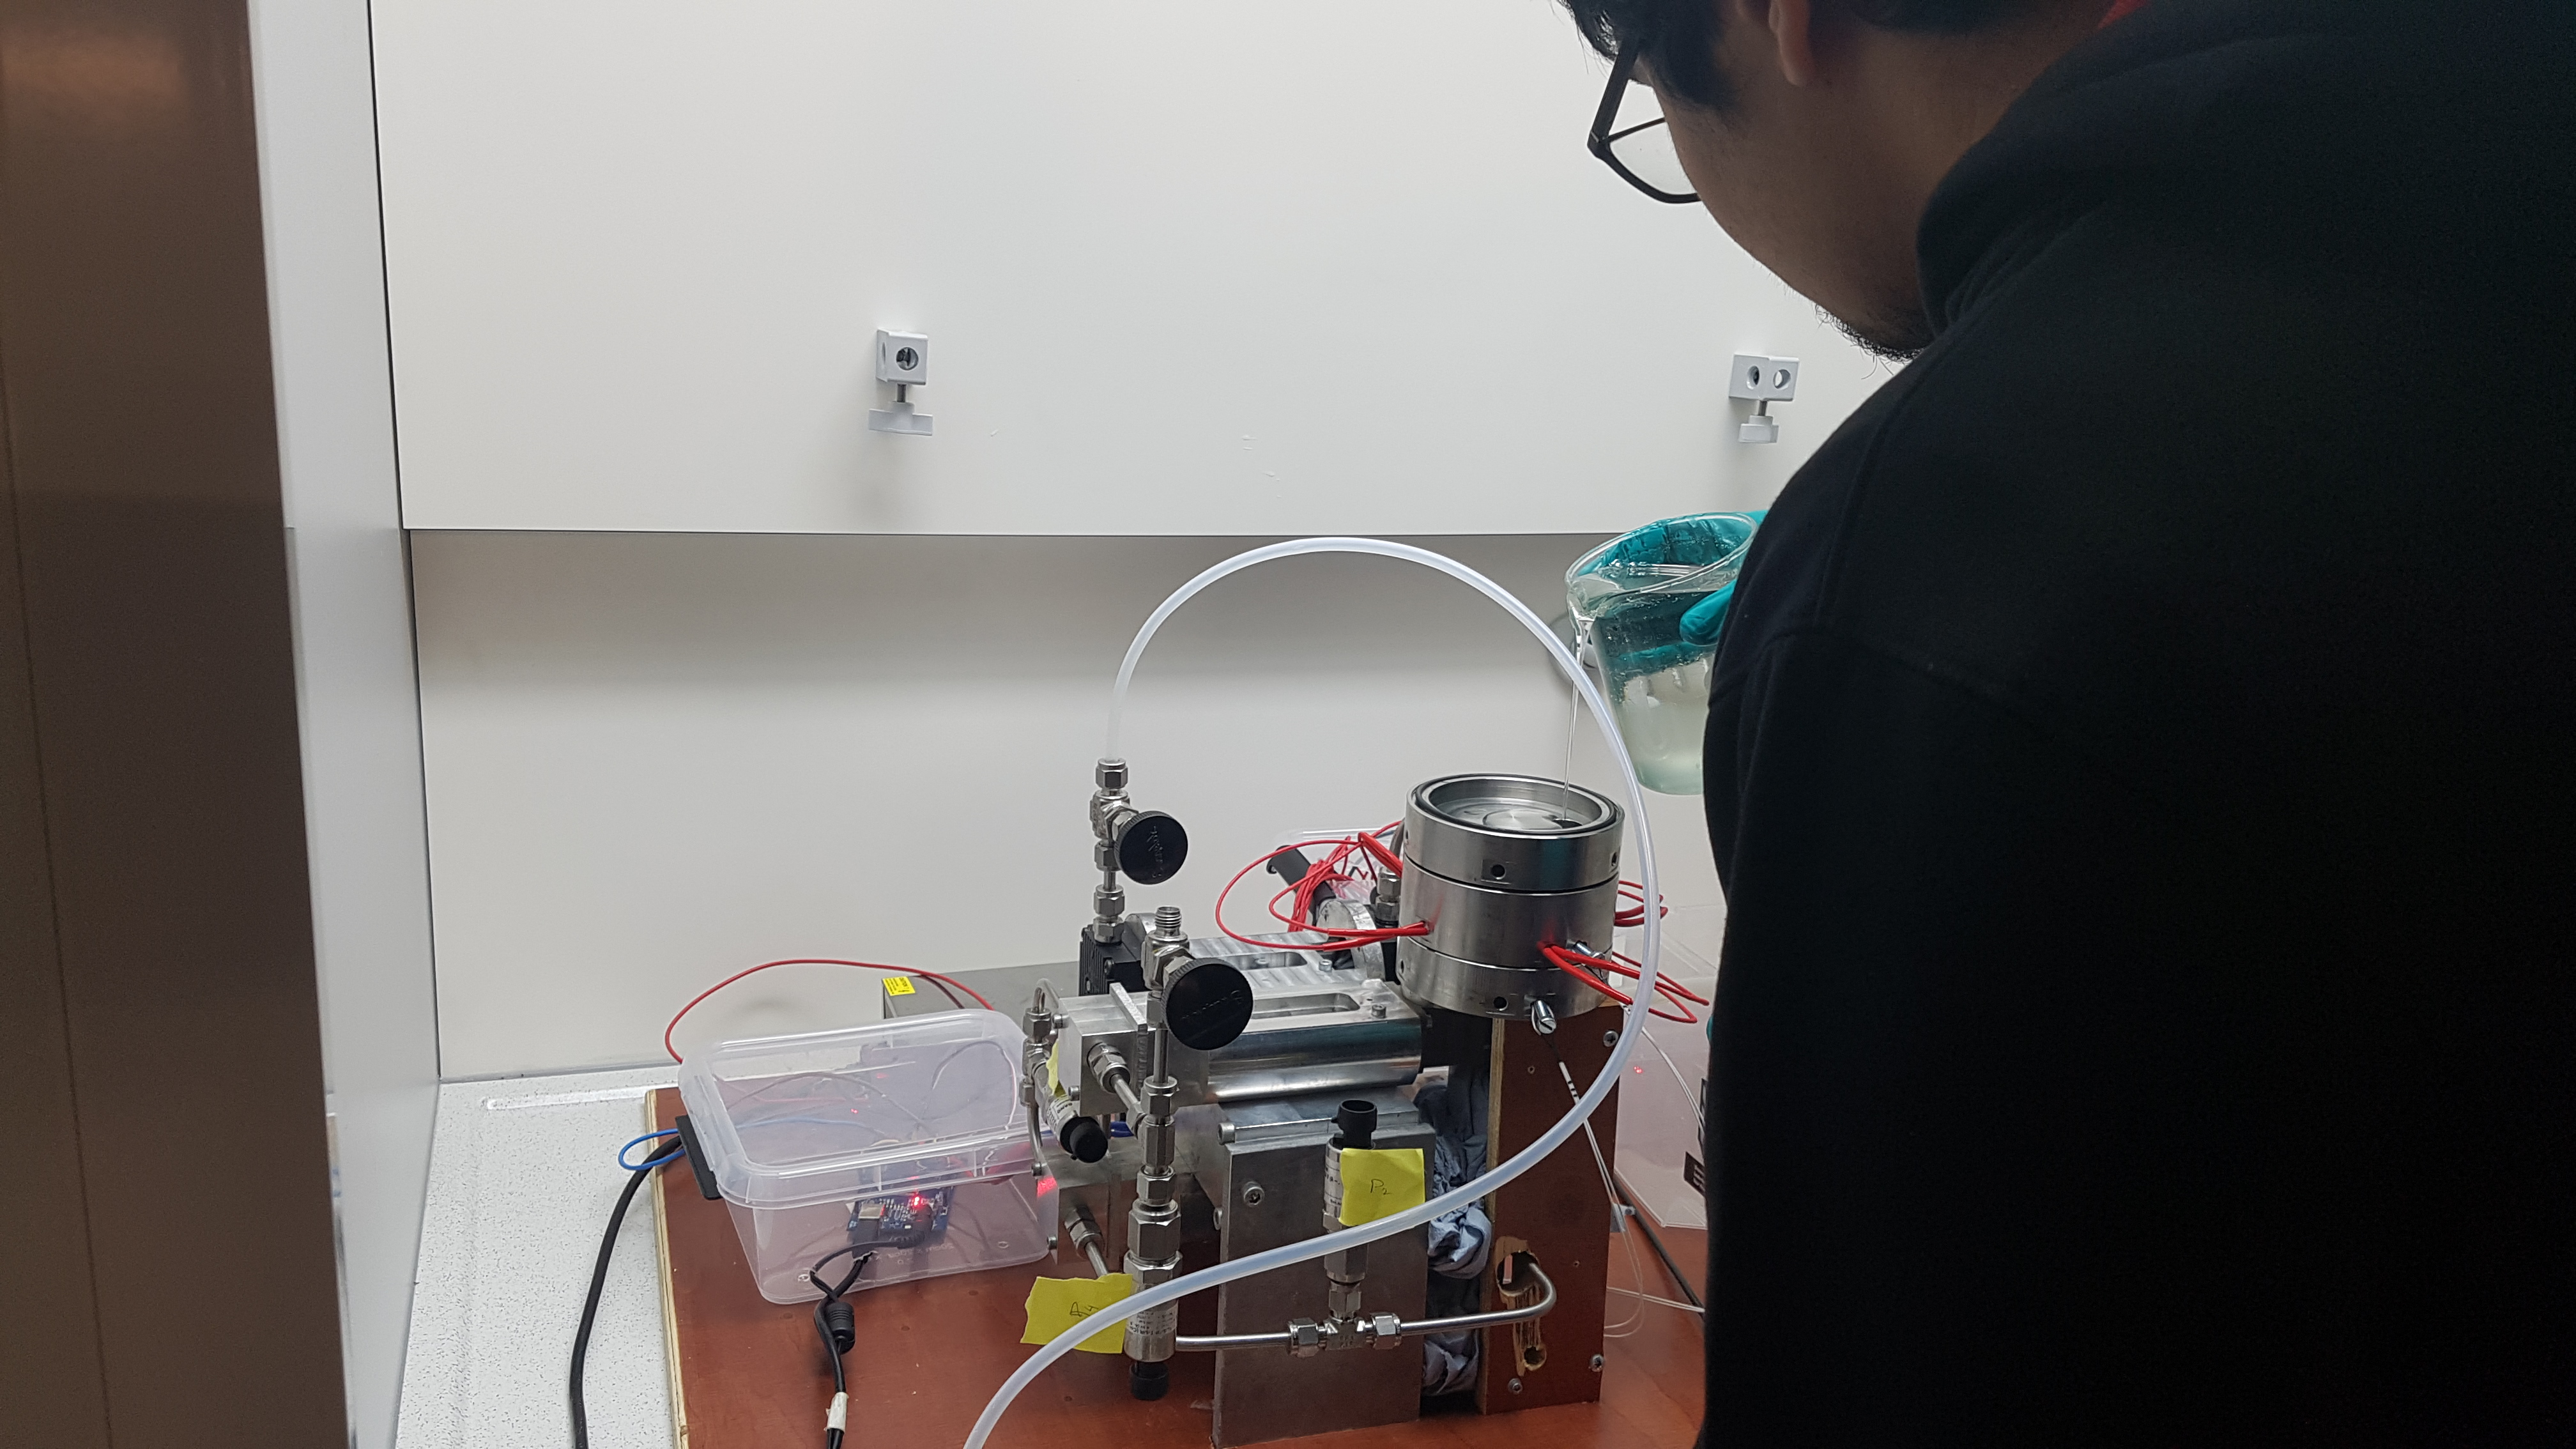
\includegraphics[scale = 0.09]{images/mywork/Sprint3/peiloading1.jpg}
    \caption{Loading PEI into the system}
    \label{fig:peiloading}
\end{figure}

It was observed that the PEI was so viscous that the PEI pump couldn't pump the normal PEI to the distributor. This was later inferred to be due to mainly two reasons :
\begin{itemize}
    \item Placement of the inlet nozzle in the extremes of the manifold - the inlet of the PEI flow from PEI pump to the DAC manifold was kept at the extreme nozzle. We know that there is significant pressure head loss when the length of pipe is very long. The solution for this was to cut the pipe length between DAC manifold and DAC distributor very short. The PEI inlet flow was shifted to the central nozzle as well for uniform distribution. 
    \item Using cold PEI - from previous reports we know that PEI becomes much less viscous at higher temperature. Hence, it wouldn't have much resistance in pumping the system up. 
\end{itemize} 


On rectifying the mistake and setting the heater temperature at 80 \degree C. The PEI was able to flow perfectly across the system and making it a continuous system. However, some observations were made that wasn't desirable which shall be elaborated more in the next Section of the report. 

\subsubsection{DAC System V1.1 breaks and issues}
\label{sec:breakdown}

During the entire runtime of the DAC System V1.1 we face many issues with broken 3D print components and leaks from the system. On further brainstorming and the cause of these issues and solutions were discussed. Some of the main issues that the system faced was : 

\begin{itemize}
    \item \textbf{Improper component geometry :} Due to improper design, improper assumptions and improper orientation. This can be seen in the following Figure \ref{fig:flowanomaly} below.
    \item \textbf{Desorber vibrations :} Due to improper orientation of the desorber chamber. At times, we could see that desorber would vibrate a lot out position and the chamber might come out of the vacuum condition. This caused a lot of PEI spills and was a pain to clean up as seen in Figure \ref{fig:leakingcompressor}. 
    
    \begin{figure}[H]
        \centering
        \begin{minipage}{.5\textwidth}
        \centering
        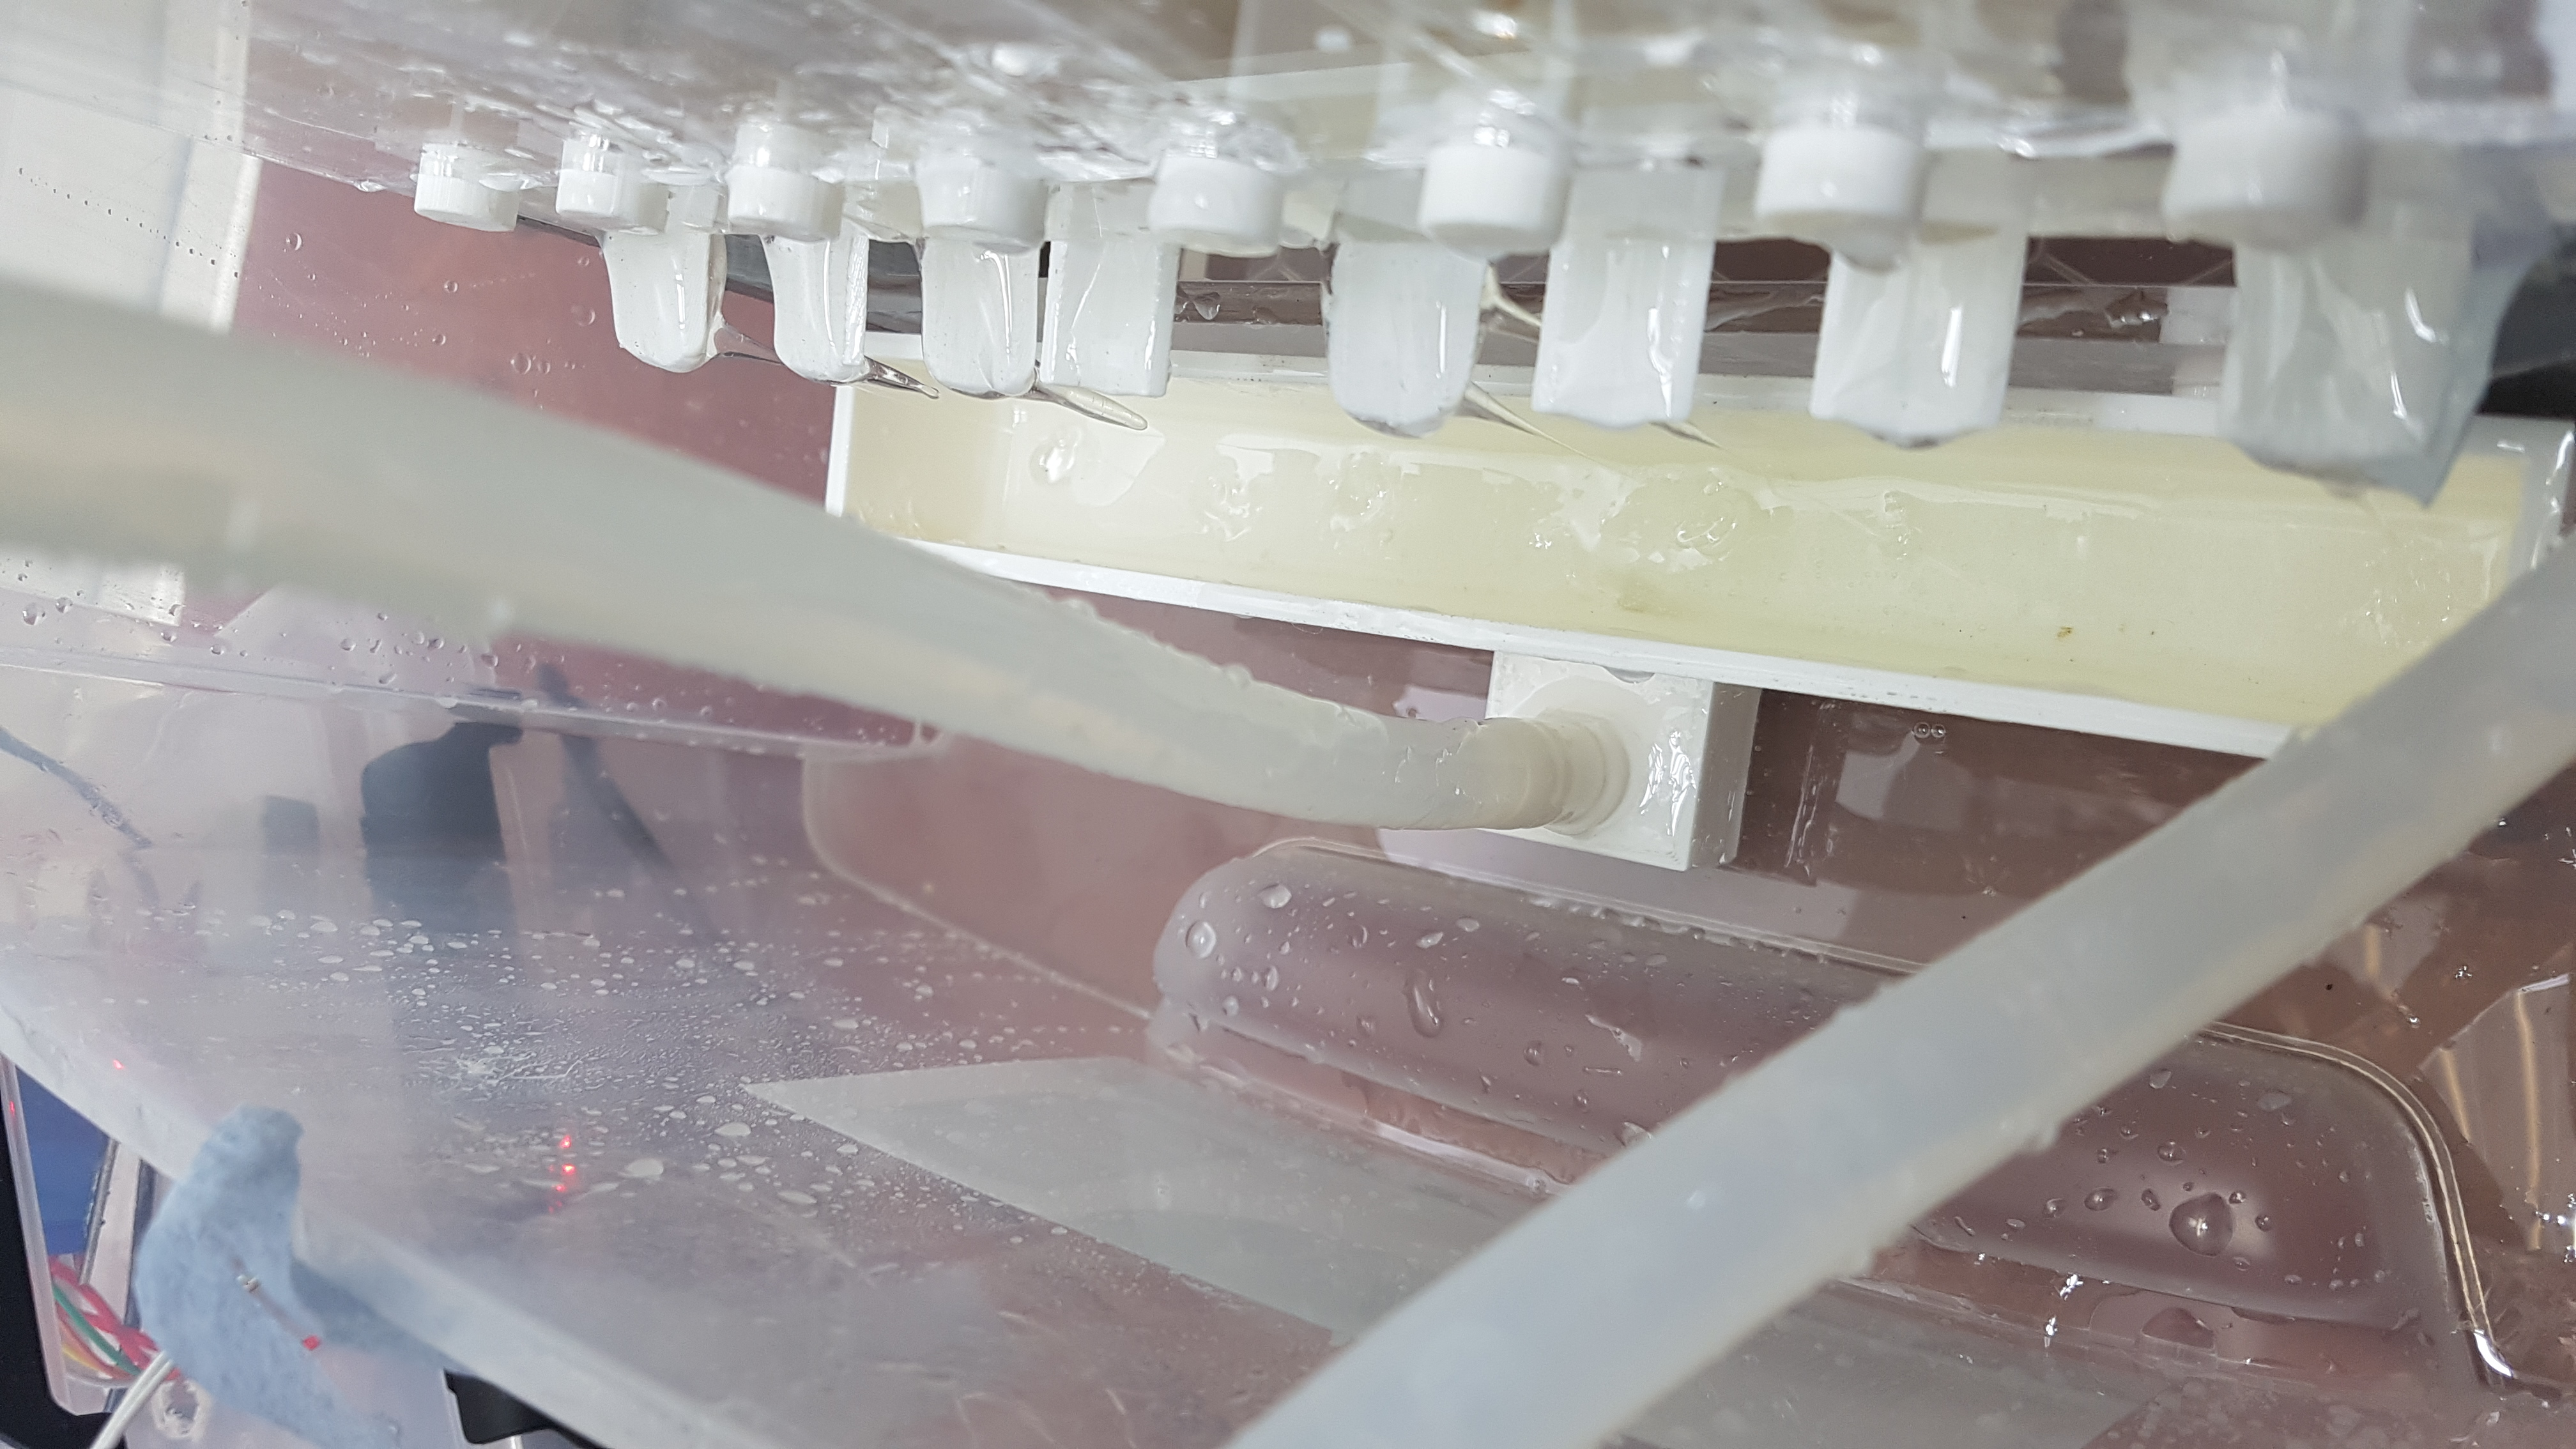
\includegraphics[width=0.9\linewidth, angle = 270]{images/mywork/Sprint3/flowanomaly.jpg}
        \captionof{figure}{Flow out of the DAC collector}
         \label{fig:flowanomaly}
    \end{minipage}%
    \begin{minipage}{.5\textwidth}
        \centering
        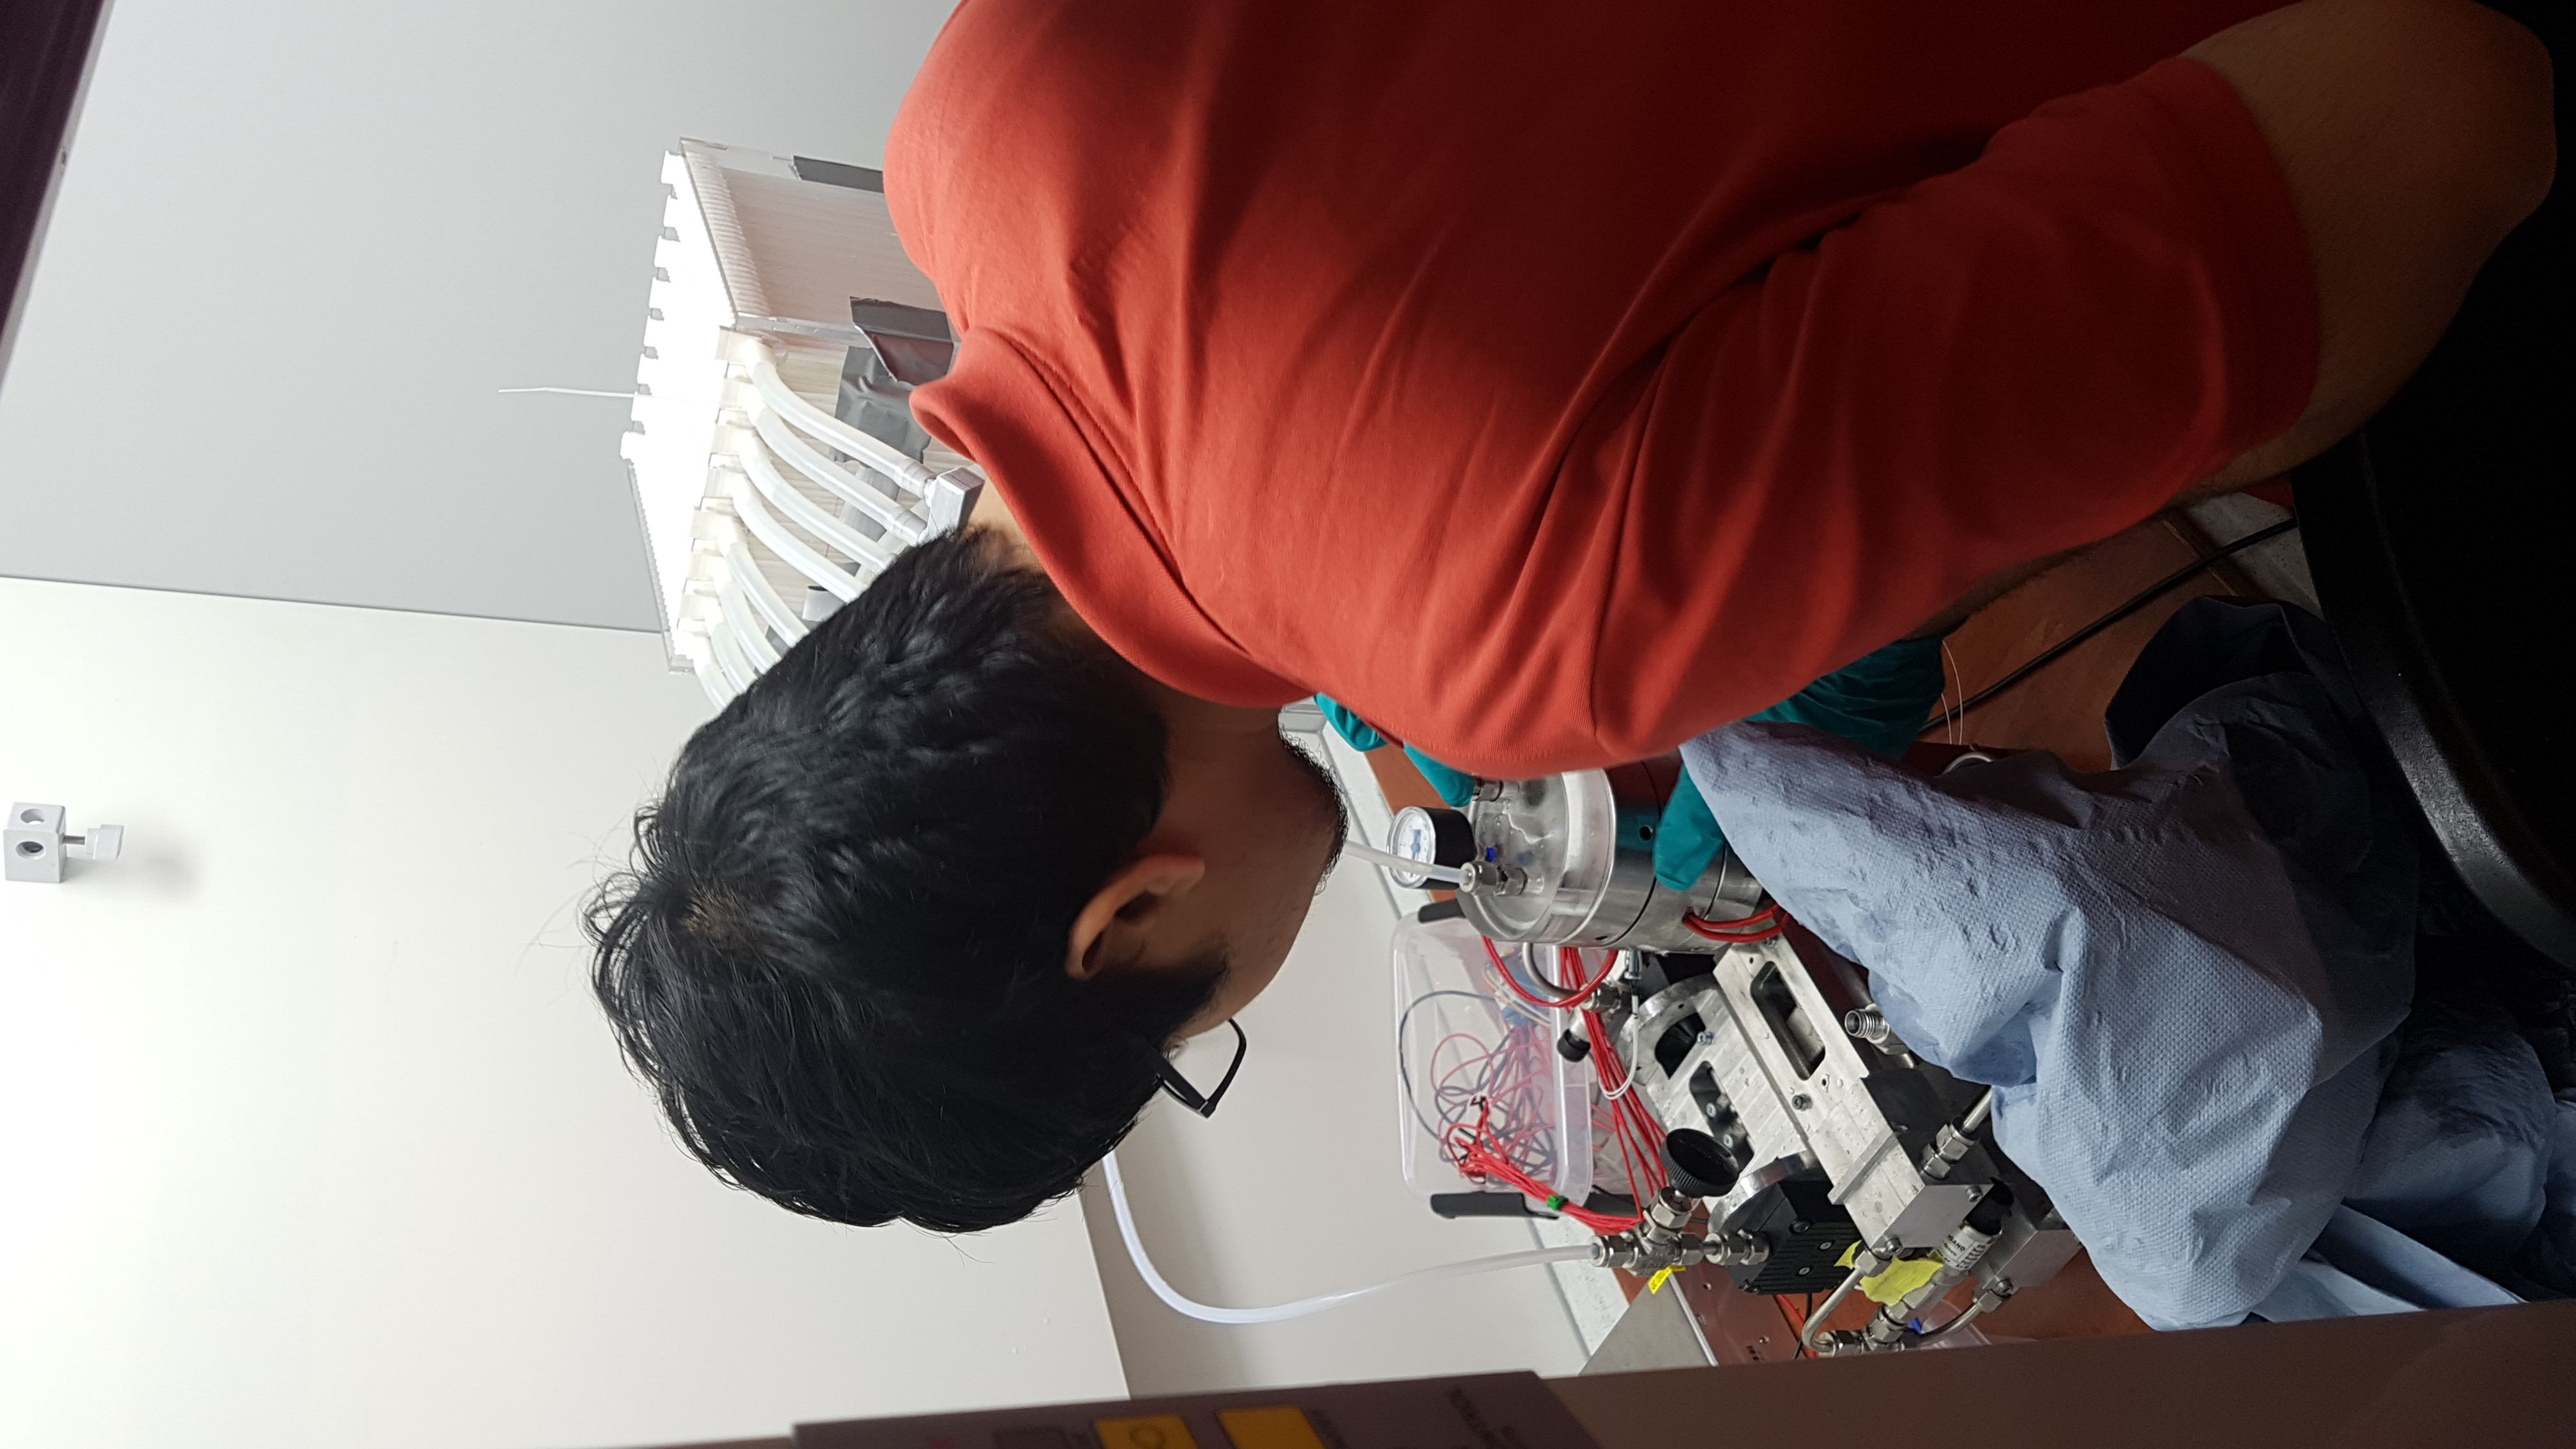
\includegraphics[width=0.9\linewidth, angle = 270]{images/mywork/Sprint3/messysystem.jpeg}
        \captionof{figure}{Leaking desorber chamber}
        \label{fig:leakingcompressor}
    \end{minipage}
    \end{figure}
    
    \item \textbf{Hot PEI reacts with PLA :}
    \label{sec:hotpei} During the Sprint 3 - a lot of our 3D prints were breaking like the collector bucket nozzle, the manifold nozzle and the distributor. At first, we inferred it was because of some accident or because of the way layers were set on the 3D printer making it a weak structure. However, on further studying it by putting a PLA piece in hot PEI. We found out that the PLA piece got completely dissolved within 30 minutes itself. Hence, it was decided that we have to look into other way to make the different DAC components.   
    
\end{itemize}


%copy paste from the section 3.3.1, section 3.3.2, section 3.4.1 and section 3.4 

\subsection{Observations from DAC V2.0 system}
\label{sec:DAC2.0}

Due to time constraints and as I was nearing the end of my internship. Further testing and running of the DAC V2.0 system was not possible. A few leak testing and tweaking the leaks were only done and has been explained below. The complete set up after assembly can be seen in Figure \ref{fig:dacv2.0} below. The labelled parts in the Figure is enumerated as per legend given below. 

\begin{enumerate}
    \item DAC V2.0 Distillation column 
    \item DAC V2.0 Absorber
    \item Vacuum pump
    \item Cooling finned tube
    \item Suction fan 
    \item DAC V2.0 Collector bucket
    \item Vacuum gauge
    \item DAC V2.0 Flowmeter
    \item T section and flashtank
\end{enumerate}

\begin{figure}[H]
    \centering
    \includegraphics[scale = 0.15]{images/mywork/Sprint5/dacv2.png}
    \caption{The DAC V2.0 system assembled}
    \label{fig:dacv2.0}
\end{figure}


\subsubsection{Vacuum leak testing}
\label{sec:DAC2.0leaks}

\noindent We found out that there is a leak in the system as the vacuum gauge wasn't staying steady once the vacuum pump was turned off. On isolating each part of the subsystem, we finalized that the issue was in the vacuum pump itself and we countered it by placing an On/Off valve right before the vacuum pump of the system. Hence, keeping the vacuum contained and operate the system in vacuum conditions. It was concluded that the leaks were mainly due to : 

\begin{itemize}
    \item \textbf{Vacuum pump:} It was found that there is were leaks present in the vacuum pump during vacuum testing. This is due to improper screwing in the male swageloke connectors. This made the leak testing difficult and was made the responsibility of the next ZEF team. 
    \item \textbf{Distillation column:} On vacuum leak testing the distillation column. We found that the vacuum pressure dropped to atmospheric pressure in a matter of few minutes. This indicated that there is leaks in the distillation column. On closer and detailed examination by leak testing each section of the distillation column. It was found that there were deep scratches in the bottom most stage. In order to overcome this, we had smoothened the surface out using sandpaper and by polishing it further using a DREMEL. 
    \item \textbf{Reboiler \& Extra feed entry:} Due to some improper welding for the swageloke connections. The vacuum couldn't be contained when the reboiler and extra feed entry in the distillation column were removed and tested seperately. Hence, they were welded again to avoid any such leaks. 
\end{itemize}


